\documentclass[11pt]{article}

\usepackage{booktabs}
\usepackage{dcolumn} 
\usepackage{epstopdf}
\usepackage{fourier}
\usepackage{fullpage}
\usepackage{graphicx}
\usepackage{hyperref}
\usepackage{longtable} 
\usepackage{natbib}
\usepackage{rotating}
\usepackage{tabularx}


\begin{document} 

\title{Here is a really great title}
\date{March 30, 2012}

\author{John J. Horton \\ oDesk Research \& Harvard Kennedy
  School\footnote{Author contact information, datasets and code are
    currently or will be available at
    \href{http://www.john-joseph-horton.com/}{http://www.john-joseph-horton.com/}.}}
\maketitle
\begin{abstract}
  Here is a really great abstract.  
\end{abstract} 

\section{Introduction}
Some people think that 
2
is an important number. 

\begin{figure}[h]
  \centering
  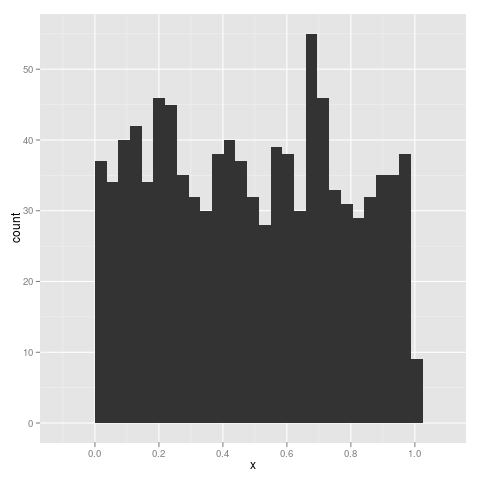
\includegraphics[scale=1]{./plots/hist.png}
  \caption{Here is a figure}
  \label{fig:hist}
\end{figure}

\bibliographystyle{aer}
\bibliography{research_tools}

\end{document} 

